\documentclass[crop,tikz,convert]{standalone}
\usetikzlibrary{positioning}

\usepackage{amsmath}
\DeclareMathAlphabet{\mbf}{OT1}{ptm}{b}{n}
\newcommand{\mbs}[1]{\ensuremath{\boldsymbol{#1}}}

\usepackage{xcolor}

\definecolor{oiorange}{rgb}{0.90, 0.60, 0.00}
\definecolor{oiskyblue}{rgb}{0.35, 0.70, 0.90}
\definecolor{oibluishgreen}{rgb}{0.00, 0.60, 0.50}
\definecolor{oigrey}{rgb}{0.60, 0.60, 0.60}

\newsavebox\state
\begin{lrbox}{\state}
    \begin{tikzpicture}[inner sep=0in, outer sep=0in]
        \node (x0) at (0.0in, 0.0in) {\includegraphics[width=6.5in]{x_0.pdf}};
        \node (x1) at (1.3in, -1.3in) {\includegraphics[width=6.5in]{x_1.pdf}};
    \end{tikzpicture}
\end{lrbox}

\newsavebox\lifted
\begin{lrbox}{\lifted}
    \begin{tikzpicture}[inner sep=0in, outer sep=0in]
        \node (th0) at ({0.6in*0}, {-0.6in*0}) {\includegraphics[width=3in]{theta_0.pdf}};
        \node (th1) at ({0.6in*1}, {-0.6in*1}) {\includegraphics[width=3in]{theta_1.pdf}};
        \node (th2) at ({0.6in*2}, {-0.6in*2}) {\includegraphics[width=3in]{theta_2.pdf}};
        \node (th3) at ({0.6in*3}, {-0.6in*3}) {\includegraphics[width=3in]{theta_3.pdf}};
        \node (th4) at ({0.6in*4}, {-0.6in*4}) {\includegraphics[width=3in]{theta_4.pdf}};
        \node (th5) at ({0.6in*5}, {-0.6in*5}) {\includegraphics[width=3in]{theta_5.pdf}};
        \node (th6) at ({0.6in*6}, {-0.6in*6}) {\includegraphics[width=3in]{theta_6.pdf}};
        \node (th7) at ({0.6in*7}, {-0.6in*7}) {\includegraphics[width=3in]{theta_7.pdf}};
        \node (th8) at ({0.6in*8}, {-0.6in*8}) {\includegraphics[width=3in]{theta_8.pdf}};
    \end{tikzpicture}
\end{lrbox}

\newsavebox\pred
\begin{lrbox}{\pred}
    \begin{tikzpicture}[inner sep=0in, outer sep=0in]
        \node[] (p) at (0, 0) {\includegraphics[width=7.8in]{pred.pdf}};
    \end{tikzpicture}
\end{lrbox}

\begin{document}
    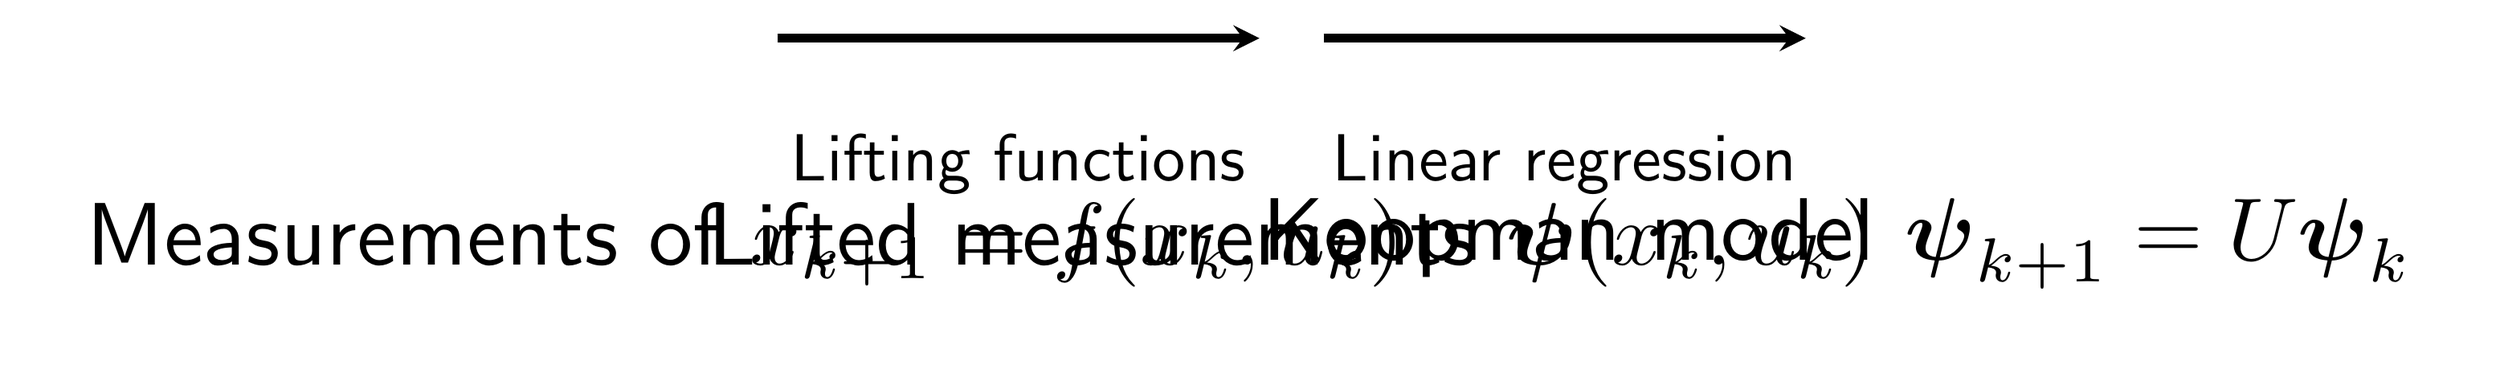
\begin{tikzpicture}[inner sep=0.1in, outer sep=0.1in, font=\sffamily]
        \node[
            label={[anchor=north, scale=4]south:Measurements of $\mbf{x}_{k + 1} = \mbf{f}(\mbf{x}_k, \mbf{u}_k)$},
        ] (x) at (0in, 0in) {\usebox{\state}};
        \node[
            right=3in of x,
            label={[anchor=north, scale=4]south:Lifted measurements $\mbs{\psi}(\mbf{x}_k, \mbf{u}_k)$},
        ] (th) {\usebox{\lifted}};
        \node[
            right=3in of th,
            label={[anchor=north, scale=4]south:Koopman model $\mbs{\psi}_{k + 1} = \mbf{U} \mbs{\psi}_k$},
        ] (pred) {\usebox{\pred}};
        \draw[
            -stealth,
            line width=4pt,
        ] (x) -- node [below, scale=3, align=center] {Lifting functions} (th);
        \draw[
            -stealth,
            line width=4pt,
        ] (th) -- node [below, scale=3, align=center] {Linear regression} (pred);
    \end{tikzpicture}
\end{document}
